%%%%%%%%%%%%%%%%%%%%%%%%%%%%%%%%%%%%%%%%%
% Programming/Coding Assignment
% LaTeX Template
%
% This template has been downloaded from:
% http://www.latextemplates.com
%
% Original author:
% Ted Pavlic (http://www.tedpavlic.com)
%
% Note:
% The \lipsum[#] commands throughout this template generate dummy text
% to fill the template out. These commands should all be removed when 
% writing assignment content.
%
% This template uses a Perl script as an example snippet of code, most other
% languages are also usable. Configure them in the "CODE INCLUSION 
% CONFIGURATION" section.
%
%%%%%%%%%%%%%%%%%%%%%%%%%%%%%%%%%%%%%%%%%

%----------------------------------------------------------------------------------------
% PACKAGES AND OTHER DOCUMENT CONFIGURATIONS
%----------------------------------------------------------------------------------------

\documentclass{scrartcl}

\usepackage{fancyhdr} % Required for custom headers
\usepackage{extramarks} % Required for headers and footers
\usepackage[usenames,dvipsnames]{color} % Required for custom colors
\usepackage{graphicx} % Required to insert images
\usepackage{listings} % Required for insertion of code
\usepackage{courier} % Required for the courier font
\usepackage{lmodern}
\usepackage[3D]{movie15}
\usepackage{hyperref}

\usepackage[backend=bibtex]{biblatex}
\addbibresource{reference.bib}

\usepackage[T1]{fontenc} % placer ici votre encodage préféré
\usepackage[utf8]{inputenc} % placer ici votre encodage préféré
\usepackage{amsmath}
\usepackage{parskip}
\newcommand{\HRule}{\rule{\linewidth}{0.5mm}}

\graphicspath{ {res/} }

% Margins
\topmargin=-0.45in
\evensidemargin=0in
\oddsidemargin=0in
\textwidth=6.5in
\textheight=9.0in
\headsep=0.25in

\linespread{1.1} % Line spacing

% Set up the header and footer
\pagestyle{fancy}
\rhead{\firstxmark} % Top right header
\lfoot{\lastxmark} % Bottom left footer
\cfoot{} % Bottom center footer
\rfoot{Page\ \thepage} 
\renewcommand\headrulewidth{0.4pt} % Size of the header rule
\renewcommand\footrulewidth{0.4pt} % Size of the footer rule

\setlength\parindent{0pt} % Removes all indentation from paragraphs



%----------------------------------------------------------------------------------------
% DOCUMENT STRUCTURE COMMANDS
% Skip this unless you know what you're doing
%----------------------------------------------------------------------------------------

% Header and footer for when a page split occurs within a problem environment
\newcommand{\enterProblemHeader}[1]{
\nobreak\extramarks{#1}{#1 continued on next page\ldots}\nobreak
\nobreak\extramarks{#1 (continued)}{#1 continued on next page\ldots}\nobreak
}

% Header and footer for when a page split occurs between problem environments
\newcommand{\exitProblemHeader}[1]{
\nobreak\extramarks{#1 (continued)}{#1 continued on next page\ldots}\nobreak
\nobreak\extramarks{#1}{}\nobreak
}


\begin{document}


%----------------------------------------------------------------------------------------
% TITLE PAGE
%----------------------------------------------------------------------------------------

\begin{titlepage}
\begin{center}

% Upper part of the page. The '~' is needed because \\
% only works if a paragraph has started.

\textsc{ Kungliga Tekniska Högskolan \\ School of Computer Science and Communication}\\[1.5cm]

\begin{figure}[ht]
\begin{center}

\includegraphics[width=0.65\textwidth]{KTH}
\end{center}
\end{figure}

\textsc{\Large DH2323}\\[0.5cm]

% Title
\HRule \\[0.4cm]
 { \huge \bfseries A Nice Title \\[0.4cm] }
{\large \bfseries  Project Documentation\\[0.4cm] }

\HRule \\[1.5cm]

% Author and supervisor
\begin{minipage}{0.65\textwidth}
\begin{flushleft} \large
Michael \textsc{Hotan} \\
Alexandre \textsc{St-Onge}\\
\end{flushleft}
\end{minipage}

\vfill

% Bottom of the page
{\large \today}

\end{center}
\end{titlepage}

%----------------------------------------------------------------------------------------
% Introduction
%----------------------------------------------------------------------------------------

\section{Introduction}

	For this project, we designed and implemented a Unity application to simulate bike traffic in a park scene. In phase 1 
	of the project we first created a park scene containing a road, park bench, trees and light sources. In phase 2 we started 
	working on the bike traffic. Finally, in phase 3 we worked on shader to apply to our cyclist model.
	
\section{Documentation}

	\subsection{Rendering a scene in Unity}
		The first step in this project was to create a realistic park scene to use as a background for our application. The simplest 
		way to do this was to use the built-in terrain feature of Unity. With the terrain object we were able to easily obtain a grassy 
		plain with trees and hill. Next we used Jacek Jankowski's street kit\parencite{Street:Jankowski} to setup a road for our future 
		bike traffic. From there, since we knew we wanted to work with some shader for our bike model, we added some street lights that 
		we got from the asset store\parencite{StreetLight:BiSkiT} and some park bench\parencite{Parkchair:Universal}. Appropriate material 
		for the sky were used with Unity's skybox to obtain a nice sky for the scene. For the daylight scenario, a single directionnal light is 
		used for the sun, while the nightime scenario uses one spotlight attached to each of the four street lights.
		
		\begin{figure}[h]
			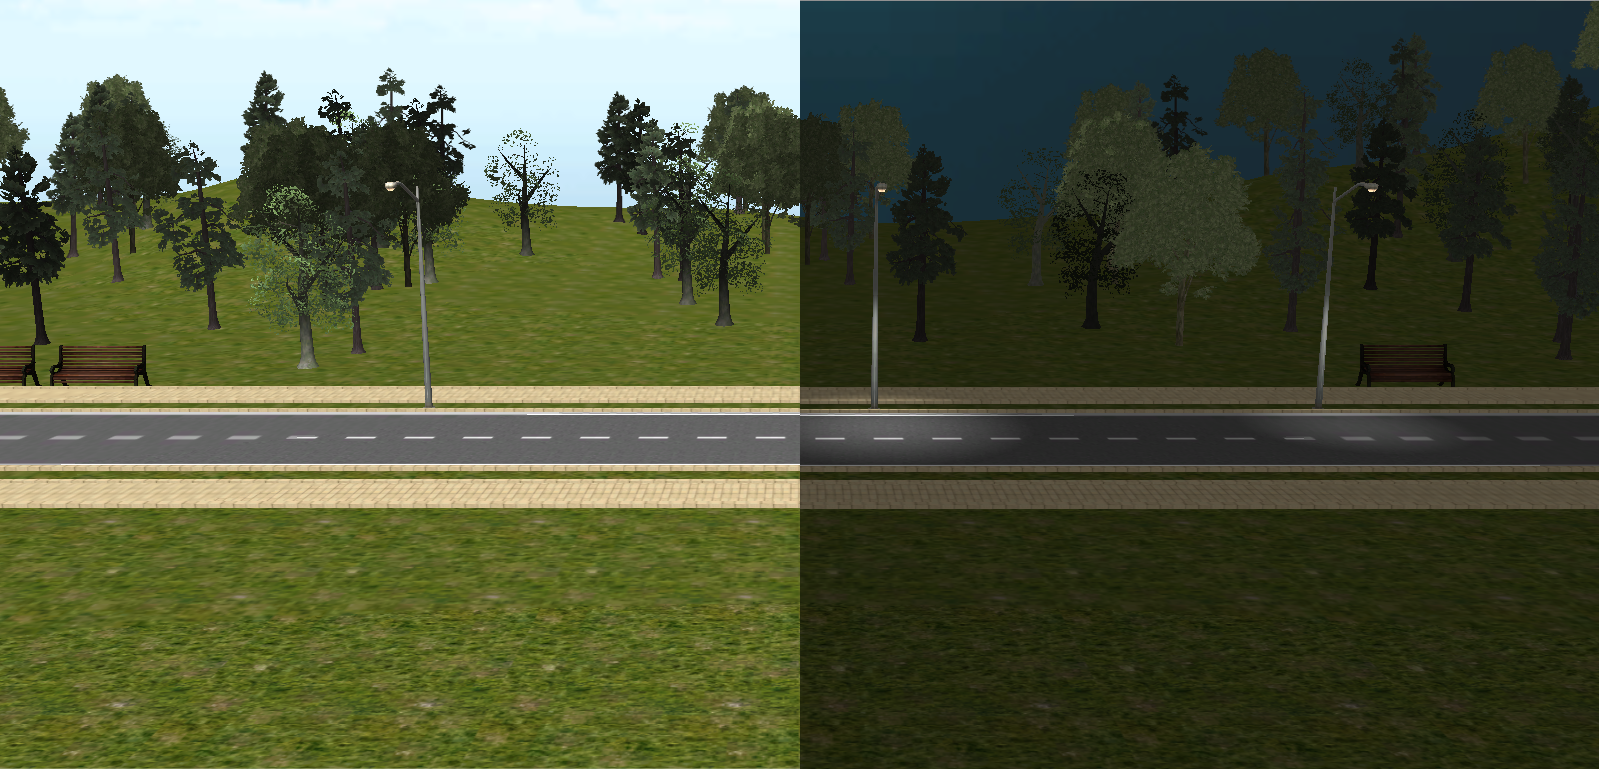
\includegraphics[width=\textwidth]{parkDayNight}
			\caption{Park scene in Unity}
			\label{fig:park_scene}
		\end{figure}
		
	\subsection{Rendering the cyclist}
		\begin{figure}[h]
			\includemovie[
				poster,
				toolbar, %same as `controls'
				label=bike2.u3d,
				text={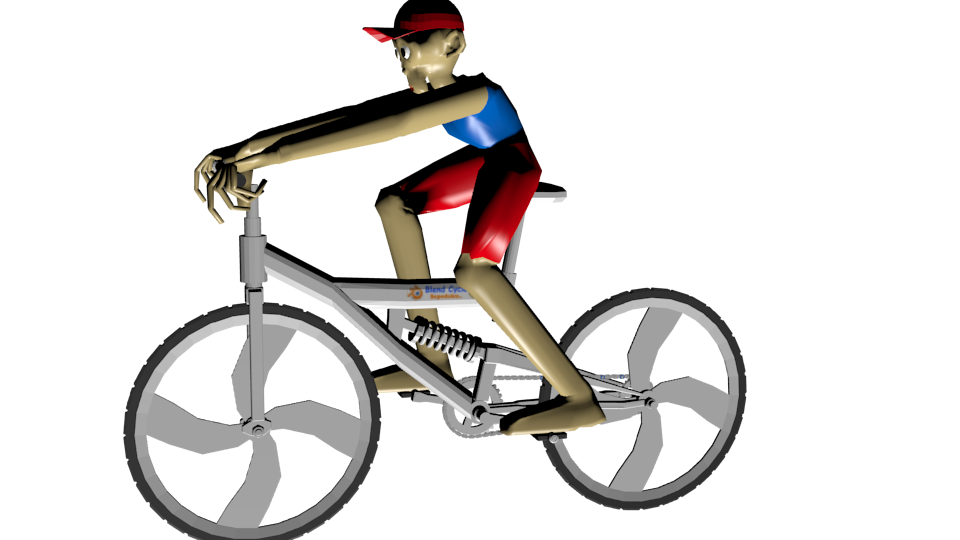
\includegraphics[width=0.8\textwidth]{BikeModel}},
				3Daac=60.000000, 3Droll=90.000000 , 3Dc2c=85.835000 60.632999 45.966000, 3Droo=42.717735, 3Dcoo=1.834687 3.523406 -1.965973,
				3Dlights=CAD,
				]{0.8\linewidth}{0.8\linewidth}{res/bike2.u3d}
			\caption{Bike 3d model found on \url{blenderswap.com}}
			\label{fig:bike_model}
		\end{figure}


\printbibliography

\end{document}

